\section{Homework 9}

\subsection{信号采样与恢复}

\subsubsection{信号的奈奎斯特频率}

(1) $f(t)$的频谱最高频率为$\omega_0/2$, 则$f(0.3t)$的频谱最高频率为$\frac{5}{3}\omega_0$, 其Nyquist频率为$\frac{10}{3}\omega_0$.

(2) $f^2(t)$的频谱最高频率为$f(t)$的两倍, 因此Nyquist频率为$2\omega_0$

(3) 时域求导相当于频域乘以$j\omega$, 不影响频谱最高频率, 其Nyquist频率仍为$\omega_0$

(4) 其频谱最高频率为$\omega_0/2+\omega_0=3\omega_0/2$, 其Nyquist频率为$3\omega_0$

(5) 其频谱为$\displaystyle F(\omega)\sum_{n=-\infty}^{+\infty}e^{-jnT_1\omega}$, 不影响信号最高频率, 因此其Nyquist频率仍为$\omega_0$.

\subsubsection{信号采样分析}

\task{第一小题}

(1) $f(t)$的频谱$F(\omega)=\frac{\pi}{2}[\delta(\omega-18\pi) + \delta(\omega-12\pi)+\delta(\omega+12\pi)+\delta(\omega+18\pi)]$.

(2) 相当于让$F(\omega)$按周期$\Omega=40\pi$变成一个周期频谱. (1)和(2)的图形如图\ref{fig:9-1-3-1}所示.

\begin{figure*}[htbp]
    \centering
    \includegraphics[width=0.7\textwidth]{images/9-1-3-1.png}
    \caption{9-1-3-1频谱}\label{fig:9-1-3-1}
\end{figure*}

(3) 应当可以保留$\delta(\omega\pm 18\pi)$的项并去除$\delta(\omega\pm 22\pi)$的项, 因此带宽的范围为$[36\pi,44\pi)$.

(4) $f_n=36\mathrm{Hz}$.

\subsection{平顶采样}

(1) 考虑一个单位冲激响应为$h(t)=f_0(t)$的LTI系统, 设$g(t)$经过时域理想采样后的结果为$g_{s1}(t)=\displaystyle
\sum_{n=\infty}^{+\infty}f(nT_s)\delta(t-nT_s)$, 则显然$g_s(t)=g_{s1}(t)*h(t)$, 因此$G_s(\omega)=\frac{1}{2\pi}
G_{s1}(\omega)H(\omega)=\displaystyle\frac{\tau}{2\pi}\operatorname{Sa}(\frac{\omega}{\tau})\sum_{n=-\infty}^{+\infty}G(\omega-n\omega_s)$.
大致频谱如图\ref{fig:9-2}所示.

\begin{figure*}[htbp]
    \centering
    \includegraphics[width=0.7\textwidth]{images/9-2.png}
    \caption{9-2频谱}\label{fig:9-2}
\end{figure*}

(2) 首先将信号做低通滤波, 得到$[-\omega_m,\omega_m]$内的频谱, 得到原信号频谱与$H(t)$的相乘结果, 因此只要将这个频谱乘以$1/H(t)$就可以.

\subsection{信号恢复补偿}

\subsubsection{采样信号恢复}

\task{必做题}

(1) 原信号频谱为$j\pi[\delta(\omega-\omega_0)-\delta(\omega+\omega_0)]$, 采样后频谱为$F_s(\omega)=\displaystyle
\sum_{n=-\infty}^{+\infty}[\delta(\omega-\omega_0-5n\omega_0)-\delta(\omega+\omega_0-5n\omega_0)]$,
将其时域卷积$u(t)-u(t-T_0/5)$, 此信号频谱为$\frac{T_0}{10}\operatorname{Sa}(\frac{\omega T_0}{20})e^{-j\omega \frac{T}{10}}$, 
则得到零阶保持的频谱: $\displaystyle\frac{T_0}{10}\operatorname{Sa}(\frac{\omega T_0}{20})e^{-j\omega\frac{T}{10}}\sum_{n=-\infty}^{+\infty}[\delta(\omega-\omega_0-5n\omega_0)-\delta(\omega+\omega_0-5n\omega_0)]$.

粗略绘制的频谱如图\ref{fig:9-3-1}.

\begin{figure*}[htbp]
    \centering
    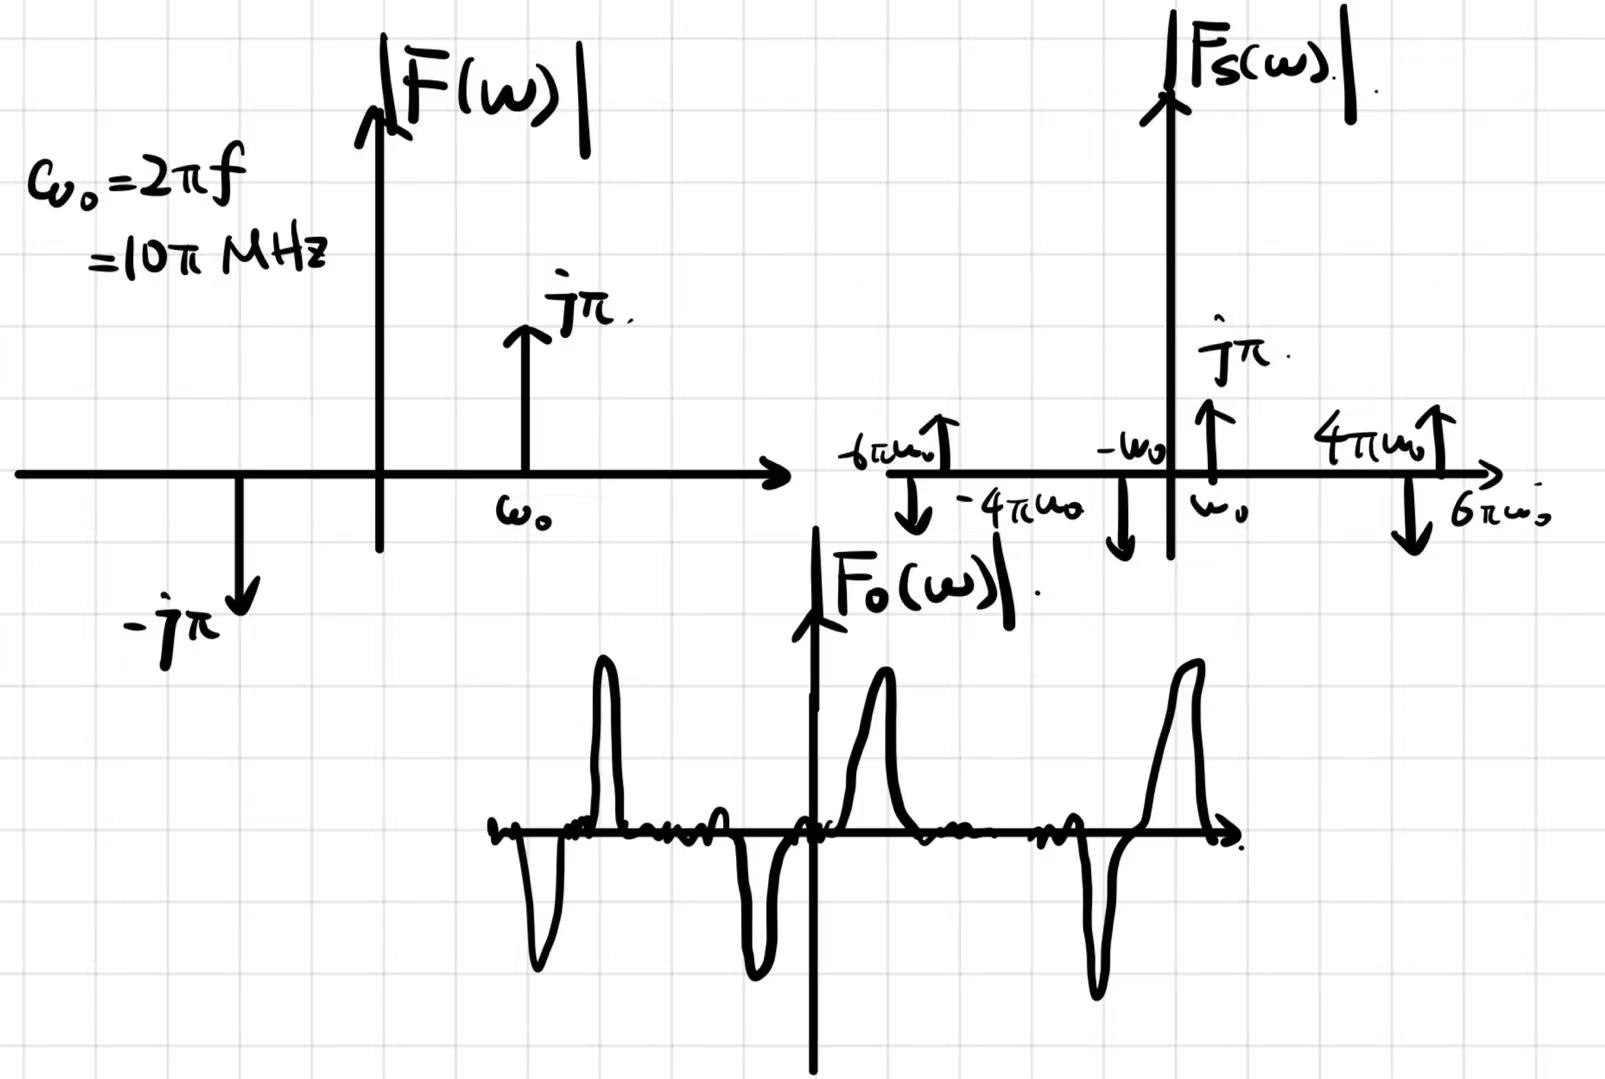
\includegraphics[width=0.7\textwidth]{images/9-3-1.jpg}
    \caption{零阶保持频谱}\label{fig:9-3-1}
\end{figure*}

(2) $H_r(\omega)=\displaystyle\left\{\begin{array}{ll}
    0,& |\omega|>25\mathrm{MHz} \\
    e^{j\omega\frac{T_0}{10}}/\operatorname{Sa}(\frac{\omega T_0}{20}),& |\omega|<25\mathrm{MHz}
\end{array}\right.$

其中$T_0=2\pi/\omega_0=\frac{2\pi}{5}\times10^{-6}\mathrm{s}$
